In this section we will be demonstrating the experimental evaluation of the Framework that we have implemented; and we will have a look at its execution time. In addition to this we will be showing the results that we obtained while collecting the data; the considered period for the collection of the data was: \emph{April 1st, 2014 - April 30th, 2014}. 


We have to have in mind that we will be considering only working days from \emph{Monday - Friday}; and if it was some holiday in this period, it was not considered in the analysis because the NYSE was close by that time.

\section{Experimental evaluation.}

In this section we will be showing the behaviour of the framework in its most important part: \emph{The Polarity Analysis}. In addition to the experimental evaluation, we have implemented \emph{multi-threading} in our framework, and we will be demonstrating experimentally how it \emph{speedup} the whole framework.

The results of the execution time of the framework for the number of words in one single thread are shown in the table \ref{tab:wordsTime} and graphically in the figure \ref{fig:wordsTime}.

\begin{figure}\centering
	\caption{Number of words vs. Execution time (ms)}\label{fig:wordsTime}
	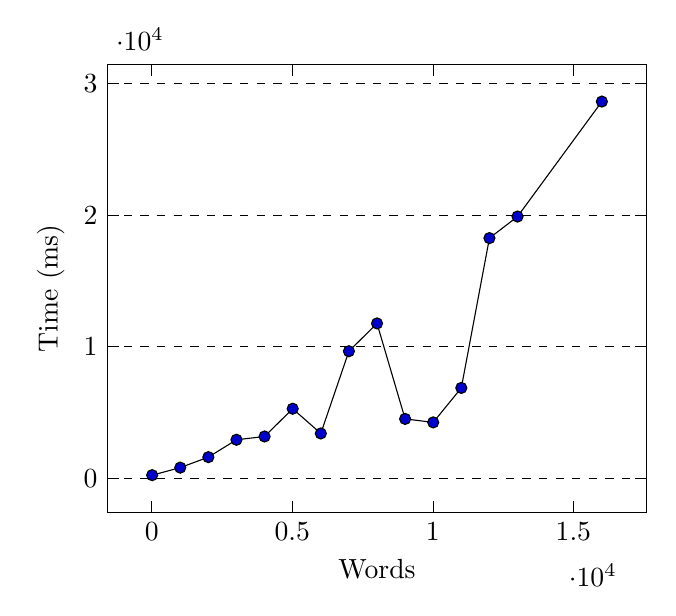
\begin{tikzpicture}
		\begin{axis}[ 
			xlabel=Words,
			ylabel=Time (ms),
			ymajorgrids=true,
			grid style=dashed,
  				]	 
			\addplot coordinates {
				(14, 229.7524129)
				(1014, 803.3164669)
				(2014, 1601.227397)
				(3014, 2921.279661)
				(4014, 3171.105263)
				(5014, 5282.681818)
				(6014, 3400.888889)
				(7014, 9654.75)
				(8014, 11768.33333)
				(9014 , 4507.2)
				(10014, 4242.875)
				(11014, 6866)
				(12014, 18255)
				(13014, 19895)
				(16014, 28639.5)
				};
		\end{axis}
	\end{tikzpicture}
\end{figure}

\begin{table}\centering
	\caption{Number of words vs. Execution time (ms)}\label{tab:wordsTime}
   	\begin{tabular}{ | p{4cm\textwidth} | p{4cm\textwidth} |}
   	\hline

\textbf{Number of Words}  & \textbf{Average Execution time (ms)}       \\\hline
14-1013     & 229.7524129 \\\hline
1014-2013   & 803.3164669 \\\hline
2014-3013   & 1601.227397 \\\hline
3014-4013   & 2921.279661 \\\hline
4014-5013   & 3171.105263 \\\hline
5014-6013   & 5282.681818 \\\hline
6014-7013   & 3400.888889 \\\hline
7014-8013   & 9654.75     \\\hline
8014-9013   & 11768.33333 \\\hline
9014-10013  & 4507.2      \\\hline
10014-11013 & 4242.875    \\\hline
11014-12013 & 6866        \\\hline
12014-13013 & 18255       \\\hline
13014-14013 & 19895       \\\hline
16014-17013 & 28639.5    \\\hline

    \end{tabular}
\end{table}


The results for the number of patterns in one single thread are shown in the table \ref{tab:patternTime} and graphically in the figure \ref{fig:patternTime}.

\begin{figure}\centering
	\caption{Number of patterns vs. Average execution time (ms)}\label{fig:patternTime}
	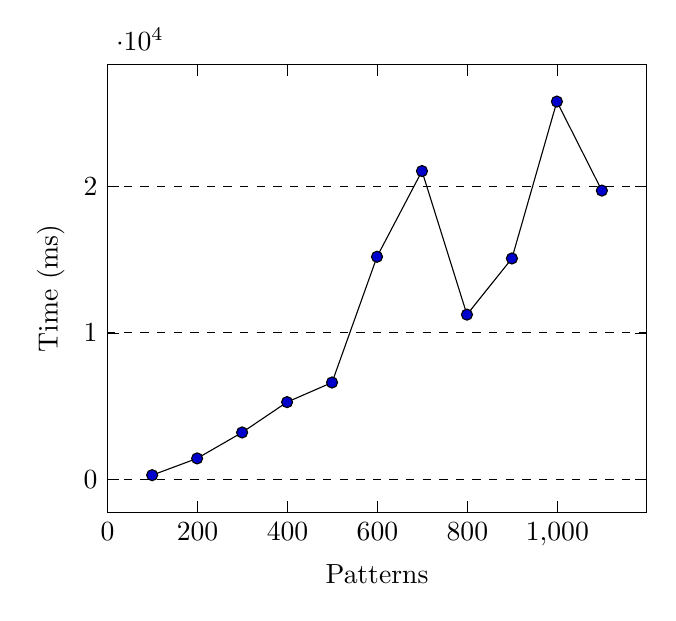
\begin{tikzpicture}
		\begin{axis}[ 
			xlabel=Patterns,
			ylabel=Time (ms),
			ymajorgrids=true,
			grid style=dashed,
  				]	 
			\addplot coordinates {
(99       , 286.5746529 )
(199    , 1430.8487   )
(299    , 3201.441441 )
(399    , 5272.302326 )
(499    , 6610.857143 )
(599    , 15193.8     )
(699    , 21042.5     )
(799    , 11245       )
(899    , 15079       )
(999    , 25786.33333 )
(1099  , 19710      )
				};
		\end{axis}
	\end{tikzpicture}
\end{figure}


\begin{table}\centering
	\caption{Number of patterns vs. Average execution time (ms)}\label{tab:patternTime}
   	\begin{tabular}{ | p{4cm\textwidth} | p{4cm\textwidth} |}
   	\hline
\textbf{Number of Patterns}  & \textbf{Average Execution time}       \\\hline
0-99       & 286.5746529 \\\hline
100-199    & 1430.8487   \\\hline
200-299    & 3201.441441 \\\hline
300-399    & 5272.302326 \\\hline
400-499    & 6610.857143 \\\hline
500-599    & 15193.8     \\\hline
600-699    & 21042.5     \\\hline
700-799    & 11245       \\\hline
800-899    & 15079       \\\hline
900-999    & 25786.33333 \\\hline
1000-1099  & 19710      \\\hline

    \end{tabular}
\end{table}

\subsection{Multi-Threading Performance}\label{MultiThreadingPerformance}

The results of the execution of the framework in several threads are presented on the table \ref{tab:threadsTime} and graphically in the figure: \ref{fig:threadsTime}. 


Taking in the theoretical background about parallel computing presented in the section \ref{ParallelComputing}, we will be mentioning the characteristics of the hardware where the tests have been performed, and after this we will be introducing the experimental results, which are shown in the table \ref{tab:threadsTime}.

\begin{itemize}
	\item CPU: 1.86 GHz Intel Core 2 Duo
	\item Memory:  4 GB, 1067 MHz DDR3
	\item Operative System: OS X 10.8.5 (12F45)
	\item Hard drive: APPLE SSD TS128C Media
	\item Considered size of the problem: \emph{n=35 patterns}
\end{itemize}

\begin{table}\centering
	\caption{Multi-Threading Performance Analysis}\label{tab:threadsTime}
   	\begin{tabular}{ | p{2.5cm\textwidth} | p{2.5cm\textwidth} | p{2.5cm\textwidth} | p{2.5cm\textwidth} | p{2.5cm\textwidth} |}
   	\hline
\textbf{Number of threads} & \textbf{Execution time (s) T(n,p)}& \textbf{Speedup S(n,p)} & \textbf{Efficiency E(n,p)} & \textbf{Cost C(n,p)} \\\hline
1               & 223.816 	&	 1			&	1			&	223.816          \\\hline
2               & 124.441	&	 1.79857121	&	0.899285605	&	248.882           \\\hline
3               & 103.705	&	 2.158198737 	&	0.719399579	&	311.115           \\\hline
4               & 111.66	&	 2.004442056	&	0.501110514	&	446.64            \\\hline
5               & 101.099	&	 2.213830008	&	0.442766002	&	505.495           \\\hline
6               & 100.934	&	 2.217449026	&	0.369574838	&	605.604           \\\hline
7               & 95.115	&	 2.353109394 	&	0.336158485	&	665.805            \\\hline
8               & 89.632	&	 2.497054623	&	0.312131828	&	717.056            \\\hline
9               & 91.493	&	 2.446263649	&	0.271807072	&	823.437            \\\hline
10              & 93.347	&	 2.397677483	&	0.239767748	&	933.47            \\\hline
11              & 124.689	&	 1.794993945	&	0.163181268	&	1371.579           \\\hline
12              & 131.235	&	 1.705459672	&	0.142121639	&	1574.82           \\\hline
13              & 134.524	&	 1.6637626	&	0.127981738	&    1748.812      \\\hline

    \end{tabular}
\end{table}

Now that we have the execution data, we will visualize each of them in a plot. \emph{Time complexity T(n,p)} \ref{ParTime} can be visualized in the figure \ref{fig:threadsTime}, \emph{Cost C(n,p)} (see: \ref{ParCost}) in the figure \ref{fig:threadsCost}, \emph{Speedup S(n,p)} (see: \ref{ParSpeedup}) in the figure \ref{fig:threadsSpeedup}, and the \emph{Efficiency E(n,p)} (see: \ref{ParEfficiency}) in the figure \ref{fig:threadsEfficiency}.

\begin{figure}\centering
	\caption{Number of threads vs Average execution time (s)}\label{fig:threadsTime}
	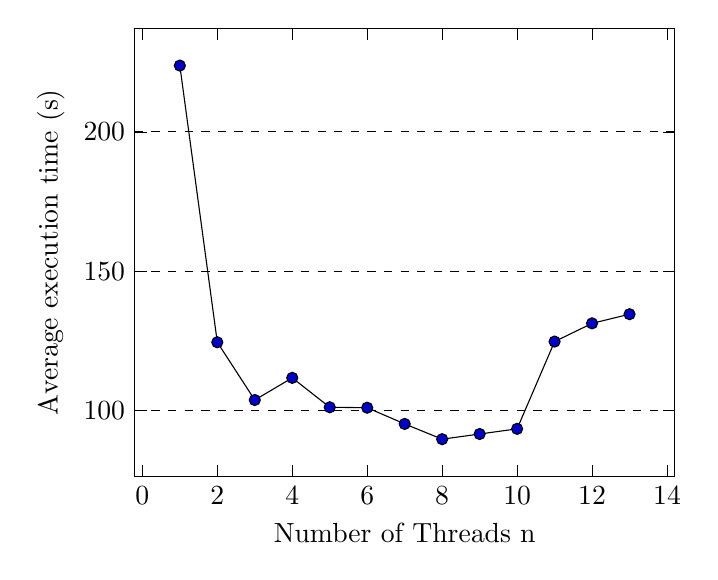
\begin{tikzpicture}
		\begin{axis}[ 
			xlabel=Number of Threads n,
			ylabel=Average execution time (s),
			ymajorgrids=true,
			grid style=dashed,
  				]	 
			\addplot coordinates {
(1               , 223.816           )
(2               , 124.441           )
(3               , 103.705           )
(4               , 111.66            )
(5               , 101.099           )
(6               , 100.934           )
(7               , 95.115            )
(8               , 89.632            )
(9               , 91.493            )
(10              , 93.347            )
(11              , 124.689           )
(12              , 131.235           )
(13              , 134.524          )
				};
		\end{axis}
	\end{tikzpicture}
\end{figure}

\begin{figure}\centering
	\caption{Number of threads vs Cost}\label{fig:threadsCost}
	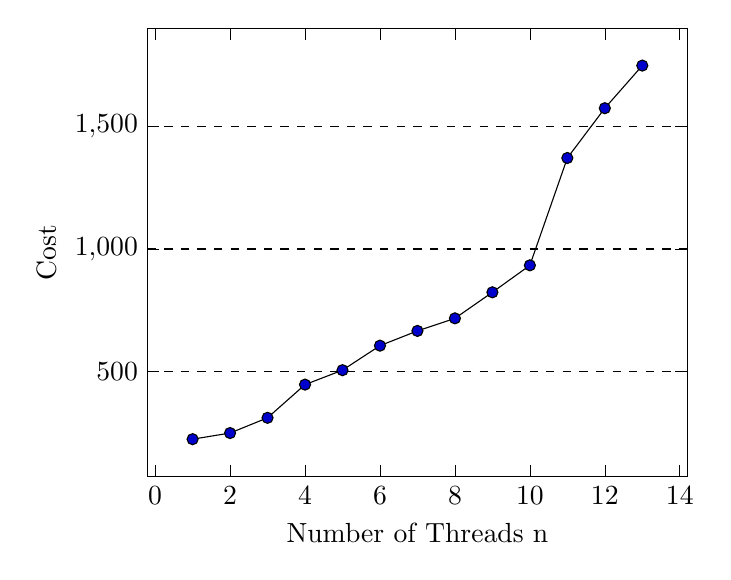
\begin{tikzpicture}
		\begin{axis}[ 
			xlabel=Number of Threads n,
			ylabel=Cost,
			ymajorgrids=true,
			grid style=dashed,
  				]	 
			\addplot coordinates {
(1               , 223.816            )
(2               , 248.882            )
(3               , 311.115           )
(4               , 446.64            )
(5               , 505.495          )
(6               , 605.604           )
(7               , 665.805            )
(8               , 717.056            )
(9               , 823.437          )
(10              , 933.47            )
(11              , 1371.579           )
(12              , 1574.82         )
(13              , 1748.812          )
				};
		\end{axis}
	\end{tikzpicture}
\end{figure}

\begin{figure}\centering
	\caption{Number of threads vs Speed up}\label{fig:threadsSpeedup}
	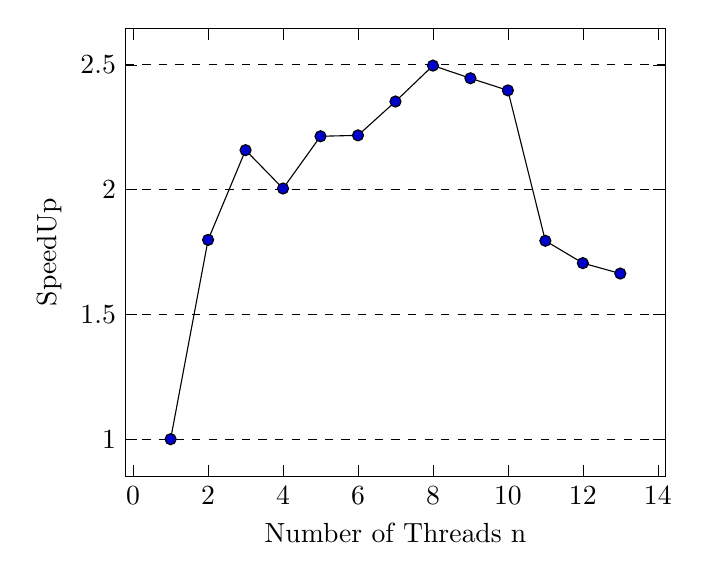
\begin{tikzpicture}
		\begin{axis}[ 
			xlabel=Number of Threads n,
			ylabel=SpeedUp,
			ymajorgrids=true,
			grid style=dashed,
  				]	 
			\addplot coordinates {
(1               , 1           )
(2               , 1.79857121  )
(3               , 2.158198737 )
(4               , 2.004442056 )
(5               , 2.213830008 )
(6               , 2.217449026 )
(7               , 2.353109394 )
(8               , 2.497054623 )
(9               , 2.446263649 )
(10              , 2.397677483 )
(11              , 1.794993945 )
(12              , 1.705459672 )
(13              , 1.6637626   )
				};
		\end{axis}
	\end{tikzpicture}
\end{figure}

\begin{figure}\centering
	\caption{Number of threads vs Efficiency}\label{fig:threadsEfficiency}
	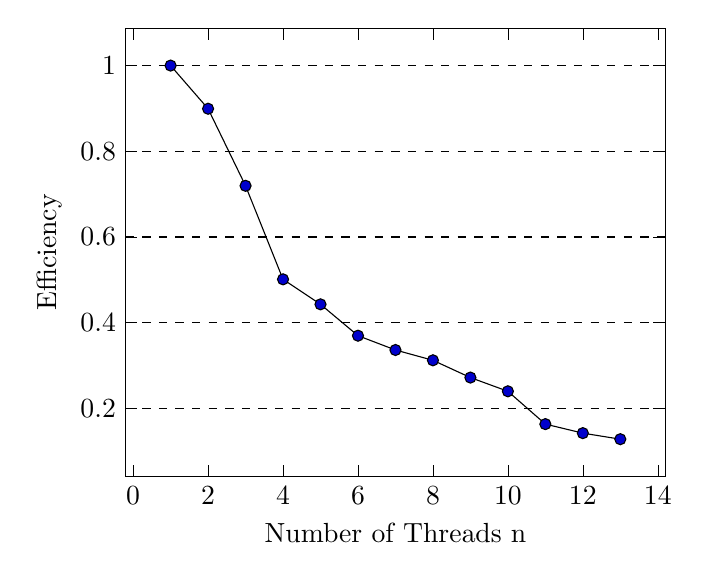
\begin{tikzpicture}
		\begin{axis}[ 
			xlabel=Number of Threads n,
			ylabel=Efficiency,
			ymajorgrids=true,
			grid style=dashed,
  				]	 
			\addplot coordinates {
(1               , 1           )
(2               , 0.899285605  )
(3               , 0.719399579 )
(4               , 0.501110514 )
(5               , 0.442766002 )
(6               , 0.369574838 )
(7               , 0.336158485 )
(8               , 0.312131828 )
(9               , 0.271807072 )
(10              , 0.239767748 )
(11              , 0.163181268  )
(12              , 0.142121639 )
(13              , 0.127981738 )
				};
		\end{axis}
	\end{tikzpicture}
\end{figure}


In order to explain our results first, we will cite Goetz \cite{SF2008} to solve our first problem: \emph{To determine the optimal number of threads that would be suitable for our task.}   For this, what we did was to run the framework with several number of threads (from 1 to 13) in our limited hardware environment, and according to the average of the results of the execution time versus the number of threads (shown in the table \ref{tab:threadsTime} and in the figure \ref{fig:threadsTime}) and the theory; there is some \emph{threshold} \cite%[p. 9]
{T2011} where when \emph{p} increases, the time decreases, but after this \emph{threshold}, the decreasing time is slower and slower with increasing \emph{p}; which means that the efficiency decreases and the cost starts to grow. Each Parallel Algorithm has its own flexibility to choose \emph{n} if \emph{p} changes or to choose \emph{p} if \emph{n} changes. After this, comes the concept of \emph{Time Scallability} (shown on the figure \ref{fig:threadsTime}), which is the minimum p, such that time is asymptotically optimal. If we analyse the figure \ref{fig:threadsTime} or the table \ref{tab:threadsTime} we can observe that after some \emph{threshold}, when adding more and more \emph{threads}, the time became worse; so after this, we will choose the number of threads that will keep a good performance without degrading the Execution time; which in our case will be 8 threads. 

Earlier we mention that we had a limited hardware environment (2 cores). And here we can see that the concurrency pay the effort. As is stated in the section \ref{concurrency}, the sequential version of our framework makes the processor \emph{iddle} for a long time, and all this time the processor is waiting for downloading or I/O operations to finish. And after implementing 8 threads, our \emph{Time T(n,p)} and \emph{Speedup S(n,p)} are maximum \emph{in our hardware environment}. 

We can conclude that this improvement makes an important impact on the performance of the framework \emph{for "free"}; because we are using exactly the same hardware. A similar behaviour would expected if we scale bigger \emph{sizes of the problem "n"} in larger \emph{infrastructures}.

\clearpage
\section{Results.}\label{ExperimentalResults1}

In order to show the results, we will present the analysed companies in the table \ref{tab:analyzedCompanies}, and we will choose one of them to analyse it a bit deeper; this company will be \emph{AAPL - Apple Inc.}, the reasons why we choose this company are simple: 
\begin{itemize}
	\item Apple now is the most valuable company in History \cite{BE2012} in terms of market capitalisation (total value of the issued shares of a publicly traded company; it is equal to the share price times the number of shares outstanding).
	\item Apple Overtakes Coca-Cola as World’s Most Valuable Brand \cite{AK2013}.
\end{itemize}
Our news crawler obtained 15,067 articles; from those 8,810 (58.47\%) were subject to heuristics, the rest 6,257 (41.52\%) articles were extracted accurately using locators as shown in the figure \ref{fig:Results1}. From this 15,067 articles 9,567 (63.50\%) were positive and 5,500 (36.50\%) were negative as shown in the figure: \ref{fig:Results2}.


\def\angle{0}
\def\radius{3}
\def\cyclelist{{"gray","silver","gray","silver","gray","silver","gray","silver"}}
\newcount\cyclecount \cyclecount=-1
\newcount\ind \ind=-1

\begin{figure}\centering

\begin{tikzpicture}[nodes = {font=\sffamily}]
  \foreach \percent/\name in {
	63.50/Positive,
	36.50/Negative
    } {
      \ifx\percent\empty\else               % If \percent is empty, do nothing
        \global\advance\cyclecount by 1     % Advance cyclecount
        \global\advance\ind by 1            % Advance list index
        \ifnum3<\cyclecount                 % If cyclecount is larger than list
          \global\cyclecount=0              %   reset cyclecount and
          \global\ind=0                     %   reset list index
        \fi
        \pgfmathparse{\cyclelist[\the\ind]} % Get color from cycle list
        \edef\color{\pgfmathresult}         %   and store as \color
        % Draw angle and set labels
        \draw[fill={\color!50},draw={\color}] (0,0) -- (\angle:\radius)
          arc (\angle:\angle+\percent*3.6:\radius) -- cycle;
        \node at (\angle+0.5*\percent*3.6:0.7*\radius) {\percent\,\%};
        \node[pin=\angle+0.5*\percent*3.6:\name]
          at (\angle+0.5*\percent*3.6:\radius) {};
        \pgfmathparse{\angle+\percent*3.6}  % Advance angle
        \xdef\angle{\pgfmathresult}         %   and store in \angle
      \fi
    };
\end{tikzpicture}


	\caption{Articles polarity.}\label{fig:Results2}
\end{figure}


\begin{figure}\centering

\begin{tikzpicture}[nodes = {font=\sffamily}]
  \foreach \percent/\name in {
	58.47/Heuristics,
	41.53/Locators
    } {
      \ifx\percent\empty\else               % If \percent is empty, do nothing
        \global\advance\cyclecount by 1     % Advance cyclecount
        \global\advance\ind by 1            % Advance list index
        \ifnum3<\cyclecount                 % If cyclecount is larger than list
          \global\cyclecount=0              %   reset cyclecount and
          \global\ind=0                     %   reset list index
        \fi
        \pgfmathparse{\cyclelist[\the\ind]} % Get color from cycle list
        \edef\color{\pgfmathresult}         %   and store as \color
        % Draw angle and set labels
        \draw[fill={\color!50},draw={\color}] (0,0) -- (\angle:\radius)
          arc (\angle:\angle+\percent*3.6:\radius) -- cycle;
        \node at (\angle+0.5*\percent*3.6:0.7*\radius) {\percent\,\%};
        \node[pin=\angle+0.5*\percent*3.6:\name]
          at (\angle+0.5*\percent*3.6:\radius) {};
        \pgfmathparse{\angle+\percent*3.6}  % Advance angle
        \xdef\angle{\pgfmathresult}         %   and store in \angle
      \fi
    };
\end{tikzpicture}

	\caption{Data extraction.}\label{fig:Results1}
\end{figure}

If we compare our results and we fix our sight on the number of articles obtained in previous works cited in the section \ref{previousResults}, we can observe that in our study, we retrieved 5.3, 2.2 and 2.7 times more articles; this results are presented in the table \ref{tab:numberArticles} and in the figure \ref{fig:Results3}. This differences in the results could be explained in the number of selected companies, sources, or merely the scope of the studies were somehow different,  among others.

\begin{table}\centering
	\caption{Number of articles}\label{tab:numberArticles}
   	\begin{tabular}{ | p{3cm\textwidth} | p{3cm\textwidth} | p{3cm\textwidth} |}
   	\hline

\textbf{Author}           & \textbf{Articles} & \textbf{Comparison} \\\hline

Schumaker \cite{SCH2012}&2,800 & 538.11\%                 \\\hline
Mittermayer \cite{MM2004}&6,600 &  228.29\%                \\\hline
Gidofalvi \cite{GG2001}& 5,500 & 273.95\%                          \\\hline

    \end{tabular}
\end{table}

\begin{figure}\centering

    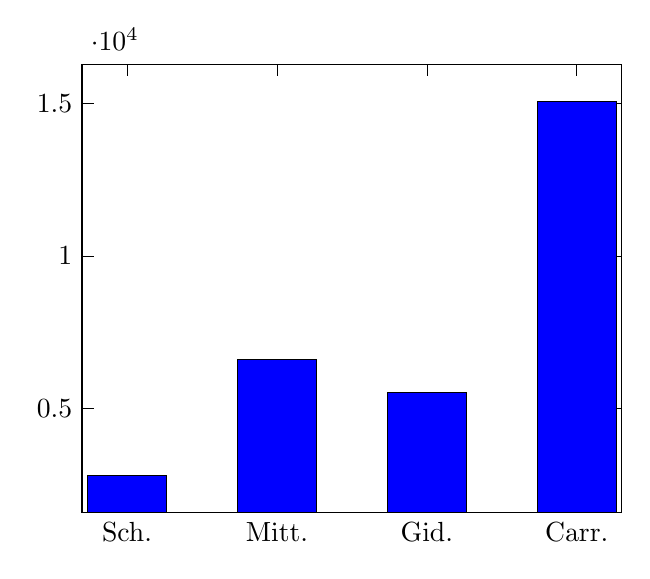
\begin{tikzpicture}
        \begin{axis}[
            symbolic x coords={Sch., Mitt., Gid., Carr.},
            xtick=data,
	  bar width=1cm
          ]
            \addplot[ybar,fill=blue] coordinates {
                (Sch.,2800)
                (Mitt.,6600)
                (Gid.,5500)
                (Carr.,15067)
            };
        \end{axis}
    \end{tikzpicture}

	\caption{Articles retrieved per Author.}\label{fig:Results3}
\end{figure}



\begin{table}\centering
	\caption{Analyzed companies}\label{tab:analyzedCompanies}
   	\begin{tabular}{ | p{3cm\textwidth} | p{7cm\textwidth} |}
   	\hline

\textbf{Symbol}           & \textbf{Name} \\\hline

AAPL   & Apple Inc.                        \\\hline
AXP    & American Express                  \\\hline
BA     & Boeing                            \\\hline
BNS    & The Nova Scotia Bank              \\\hline
CAT    & Caterpillar                       \\\hline
CSCO   & Cisco                             \\\hline
CVX    & Chevron                           \\\hline
DD     & Du Pont                           \\\hline
DIS    & The Walt Disney Company           \\\hline
GE     & General Electric                  \\\hline
GS     & Goldman Sachs Group               \\\hline
HD     & Home Depot                        \\\hline
HMC    & Honda Motor                       \\\hline
IBM    & IBM                               \\\hline
INTC   & Intel                             \\\hline
JNJ    & Johnson \& Johnson                \\\hline
JPM    & JPMorgan Chase                    \\\hline
KO     & Coca Cola                         \\\hline
MCD    & McDonald's                        \\\hline
MMM    & 3M                                \\\hline
MRK    & Merck                             \\\hline
MSFT   & Microsoft                         \\\hline
NKE    & Nike                              \\\hline
OXY    & Occidental Petroleum Corporation  \\\hline
PBR    & Petróleo Brasileiro - Petrobras   \\\hline
PFE    & Pfizer                            \\\hline
PG     & Procter \& Gamble                 \\\hline
T      & AT\&T                             \\\hline
TRV    & Travelers Companies               \\\hline
UNH    & United Health Companies           \\\hline
UTX    & United Technologies Corp          \\\hline
V      & Visa                              \\\hline
VZ     & Verizon Communications            \\\hline
WMT    & Wal-Mart                          \\\hline
XOM    & Exxon Mobil                       \\\hline
YPF    & Yacimientos Petrolíferos Fiscales \\\hline

    \end{tabular}
\end{table}

First of all we will analyse the correlation of the chosen company in the previously mentioned period (\emph{April 1st, 2014 - April 30th, 2014}). But before that, we must make a reference to the \emph{Pearson correlation coefficient} mentioned in \ref{PearsonCorr}. Now, we will proceed to interpret the obtained data. We will start with the table \ref{tab:ResultsApple} which shows the news articles (positive and negative), the price and delta (variation of the current price according to the price of the day before). And if we apply the \emph{Pearson correlation coefficient} to the \emph{Number of positive articles} and to \emph{Price delta} we would get: \emph{r = -37.83\%} and when we correlate the \emph{Number of negative articles} and the \emph{Price delta} we get \emph{r = -37.85\%}. According to this numbers and to the interpretation of the coefficient; first thing that we can observe is that both numbers have the same direction and they are very close to each other, so this means that in this period if they have good news, their price will somehow drop, and if they have bad news, their price as well will drop, and the negative news will have more impact than the positive ones, as we could contrast with real life, when Apple has bad news, its reputation goes down and it directly affect the price of the stock.


\begin{table}\centering
	\caption{Results AAPL}\label{tab:ResultsApple}
   	\begin{tabular}{ | p{2cm\textwidth} | p{2cm\textwidth} | p{2cm\textwidth} | p{2cm\textwidth} | p{2.5cm\textwidth} |}
   	\hline

\textbf{Date}           & \textbf{Positive} & \textbf{Negative} & \textbf{Price}  & \textbf{PriceDelta\$} \\
01/04/14& 14       & 15       & 541.65 & 4.910035584  \\\hline
02/04/14& 38       & 15       & 542.55 & 0.899965664  \\\hline
03/04/14& 31       & 14       & 538.79 & -3.76001067  \\\hline
04/04/14& 34       & 13       & 531.82 & -6.969979738 \\\hline
07/04/14& 34       & 17       & 523.47 & -8.350027011 \\\hline
08/04/14& 22       & 13       & 523.44 & -0.029968249 \\\hline
09/04/14& 22       & 16       & 530.32 & 6.880000456  \\\hline
10/04/14& 22       & 7        & 523.48 & -6.84005142  \\\hline
11/04/14& 9        & 5        & 519.61 & -3.869992927 \\\hline
14/04/14& 17       & 7        & 521.68 & 2.070005373  \\\hline
15/04/14& 15       & 10       & 517.96 & -3.719968002 \\\hline
16/04/14& 10       & 6        & 519.01 & 1.049988371  \\\hline
17/04/14& 13       & 1        & 524.94 & 5.92998471   \\\hline
21/04/14& 12       & 9        & 531.17 & 6.23         \\\hline
22/04/14& 16       & 16       & 531.7  & 0.530029399  \\\hline
23/04/14& 14       & 12       & 524.75 & -6.9499989   \\\hline
24/04/14& 4        & 3        & 567.77 & 43.01998968  \\\hline
25/04/14& 1        & 5        & 571.94 & 4.169980224  \\\hline
28/04/14& 15       & 7        & 594.09 & 22.15005156  \\\hline
29/04/14& 8        & 7        & 592.33 & -1.760007899 \\\hline
30/04/14& 1        & 5        & 590.09 & -2.239987541 \\\hline

    \end{tabular}
\end{table}

In the table \ref{tab:ResultsApple}, we focused in a period of one month, here is presented the correlation coefficient in a weekly basis. And as we can see, the weekly correlations are quite different between each others and the negative correlations appear several times in the analysis.

\begin{table}\centering
	\caption{AAPL Weekly correlation}\label{tab:ResultsApple}
   	\begin{tabular}{ | p{1.8cm\textwidth} | p{1cm\textwidth} | p{1cm\textwidth} | p{1.1cm\textwidth} | p{1.1cm\textwidth} | p{2.5cm\textwidth} | p{2.5cm\textwidth} |}
   	\hline

\textbf{Date}           & \textbf{Pos.} & \textbf{Neg.} & \textbf{Price}  & \textbf{Delta (\$)} & \textbf{Pos.-price corr.} & \textbf{Neg-price corr.} \\\hline
01/04/14 & 14   & 15   & 541.65 & 4.91         &                    &                     \\\hline
02/04/14 & 38   & 15   & 542.55 & 0.90         &                    &                     \\\hline
03/04/14 & 31   & 14   & 538.79 & -3.76        &                    &                     \\\hline
04/04/14 & 34   & 13   & 531.82 & -6.97        & -0.645596372       & 0.935331709         \\\hline
07/04/14 & 34   & 17   & 523.47 & -8.35        &                    &                     \\\hline
08/04/14 & 22   & 13   & 523.44 & -0.03        &                    &                     \\\hline
09/04/14 & 22   & 16   & 530.32 & 6.88         &                    &                     \\\hline
10/04/14 & 22   & 7    & 523.48 & -6.84        &                    &                     \\\hline
11/04/14 & 9    & 5    & 519.61 & -3.87        & -0.242402973       & 0.321685525         \\\hline
14/04/14 & 17   & 7    & 521.68 & 2.07         &                    &                     \\\hline
15/04/14 & 15   & 10   & 517.96 & -3.72        &                    &                     \\\hline
16/04/14 & 10   & 6    & 519.01 & 1.05         &                    &                     \\\hline
17/04/14 & 13   & 1    & 524.94 & 5.93         & -0.177342173       & -0.95274704         \\\hline
21/04/14 & 12   & 9    & 531.17 & 6.23         &                    &                     \\\hline
22/04/14 & 16   & 16   & 531.7  & 0.53         &                    &                     \\\hline
23/04/14 & 14   & 12   & 524.75 & -6.95        &                    &                     \\\hline
24/04/14 & 4    & 3    & 567.77 & 43.02        &                    &                     \\\hline
25/04/14 & 1    & 5    & 571.94 & 4.17         & -0.549262067       & -0.715444882        \\\hline
28/04/14 & 15   & 7    & 594.09 & 22.15        &                    &                     \\\hline
29/04/14 & 8    & 7    & 592.33 & -1.76        &                    &                     \\\hline
30/04/14 & 1    & 5    & 590.09 & -2.24        & 0.874501955        & 0.514829914    \\\hline    

    \end{tabular}
\end{table}

Finally, we present the correlations between positive and negative articles with the delta price. We can observe in the table \ref{tab:GeneralResults} that the same pattern that we had in the correlation of the data of the table \ref{tab:sectionApple} repeats here. Not in every case, but usually both numbers are somehow close to each other and that news articles are not the only factor that affects the changes in the price of a stock. In this case, we should look for another approaches how to analyse the data, as we will recommend in the next section. Now that we have a sample of news, more complex data analysis techniques should be applied, which is out of the scope of this work.

\begin{table}\centering
	\caption{Results of the correlations for each analyzed company}\label{tab:GeneralResults}
   	\begin{tabular}{ | p{2cm\textwidth} | p{3.5cm\textwidth} | p{3.5cm\textwidth} | p{3.5cm\textwidth} | }
   	\hline
\textbf{Company} & \textbf{Positve-Delta Price} & \textbf{Negative-Delta Price} & \textbf{Difference (abs)}  \\\hline
AAPL    & -37.83\%           & -37.85\%            & -0.02\%  \\\hline
AXP     & -42.30\%           & -41.30\%            & 1.00\%   \\\hline
BA      & -37.82\%           & -30.10\%            & 7.72\%   \\\hline
BNS     & -6.64\%            & -14.41\%            & -7.77\%  \\\hline
CAT     & 14.64\%            & 29.17\%             & -14.52\% \\\hline
CAT     & -16.68\%           & -24.23\%            & -7.55\%  \\\hline
CVX     & -21.48\%           & -20.04\%            & 1.43\%   \\\hline
DD      & -20.96\%           & -32.00\%            & -11.04\% \\\hline
DIS     & -21.40\%           & -28.47\%            & -7.08\%  \\\hline
GE      & -44.37\%           & -38.52\%            & 5.85\%   \\\hline
GS      & -71.09\%           & -88.32\%            & -17.23\% \\\hline
HD      & -32.88\%           & -23.42\%            & 9.46\%   \\\hline
HMC     & -11.01\%           & -8.32\%             & 2.69\%   \\\hline
IBM     & 4.53\%             & 18.44\%             & -13.91\% \\\hline
IBM     & 10.52\%            & -4.29\%             & 6.23\%   \\\hline
JNJ     & -10.87\%           & -9.28\%             & 1.60\%   \\\hline
JPM     & -40.92\%           & -66.41\%            & -25.49\% \\\hline
KO      & -4.39\%            & 13.24\%             & -8.84\%  \\\hline
MCD     & -16.50\%           & -23.79\%            & -7.29\%  \\\hline
MMM     & -6.10\%            & -3.51\%             & 2.59\%   \\\hline
MRK     & -41.52\%           & 0.49\%              & 41.03\%  \\\hline
MSFT    & -12.49\%           & -9.19\%             & 3.30\%   \\\hline
NKE     & 12.13\%            & 23.71\%             & -11.57\% \\\hline
OXY     & -5.87\%            & -2.57\%             & 3.30\%   \\\hline
PFE     & -23.42\%           & -23.69\%            & -0.27\%  \\\hline
PG      & 0.47\%             & 15.96\%             & -15.49\% \\\hline
T       & -3.97\%            & -19.42\%            & -15.45\% \\\hline
TRV     & -5.67\%            & -2.87\%             & 2.80\%   \\\hline
UNH     & -25.98\%           & -40.06\%            & -14.08\% \\\hline
UTX     & -35.10\%           & -48.49\%            & -13.38\% \\\hline
V       & -5.73\%            & -25.02\%            & -19.29\% \\\hline
VZ      & -0.43\%            & -6.19\%             & -5.75\%  \\\hline
WMT     & 3.37\%             & -30.49\%            & -27.13\% \\\hline
XOM     & -38.55\%           & -29.69\%            & 8.86\%   \\\hline
YPF     & 26.45\%            & 18.48\%             & 7.97\%  \\\hline

    \end{tabular}
\end{table}


